\documentclass[tikz,border=2]{standalone}
\usepackage{amssymb}
\usetikzlibrary{shadows,arrows,shapes,positioning,calc,backgrounds,fit}
\begin{document}

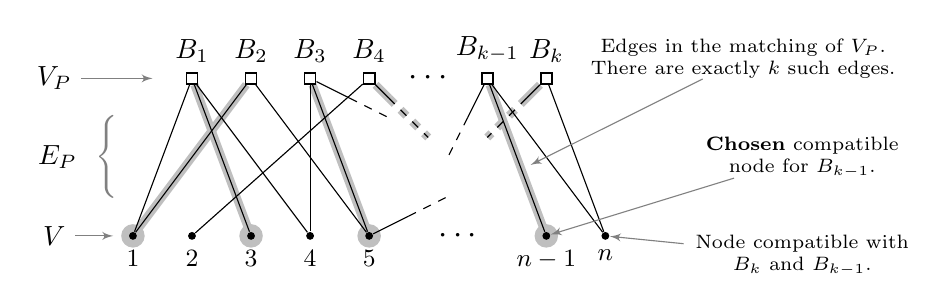
\begin{tikzpicture}
[scale=1,transform shape,
node distance=1cm,
%
vertex/.style={shape=circle,fill=black,inner sep=1pt},
selected/.style={shape=circle,fill=black!25,inner sep=3pt},
part/.style={shape=rectangle,draw=black,inner sep=2pt,semithick},
%
every edge/.style={draw,thin},
match/.style={draw,line width=3pt,black!25},
dedge/.style={>=latex', shorten >=.0pt, shorten <=.0pt, thin, black!50}]
%
% V_P
\foreach \x in {1,...,4}
   \node (B\x) [part,label=above:$B_{\x}$] at (.75*\x,2) {};
%%
\node at (.75*5,2) {\large $\cdots$};
\node (Bkm) [part,label=above:$B_{k-1}$] at (.75*6,2) {};
\node (Bk) [part,label=above:$B_{k}$] at (.75*7,2) {};
%%
% V
\foreach \x in {1,...,5}
\node (v\x) [vertex,label=below:{\small $\x$}] at (.75*\x-.75,0) {};
\node at (.75*5.5,0) {\large $\cdots$};
\node (vnm) [vertex,label=below:{\small ${n-1}$}] at (.75*7,0) {};
\node (vn) [vertex,label=below:{\small ${n}$}] at (.75*8,0) {};
%%
% all edges
%%% matched edges
\draw (B1) -- (v3);
\draw (B2) -- (v1);
\draw (B3) -- (v5);
\draw (B4) -- +(.25,-.25);
\draw[dashed] (B4)+(.25,-.25) -- +(.75,-.75);
\draw (Bkm) -- (vnm);
\draw (Bk) -- +(-.25,-.25);
\draw[dashed] (Bk)+(-.25,-.25) -- +(-.75,-.75);
%% other edges
\draw (B1) -- (v1);
\draw (B1) -- (v4);
\draw (B2) -- (v5);
\draw (B3) -- (v4);
\draw (B3) -- +(.5,-.25);
\draw[dashed] (B3)+(.5,-.25) -- +(1,-.5);
\draw (B4) -- (v2);
\draw (Bkm) -- +(-.25,-.5);
\draw[dashed] (Bkm)+(-.25,-.5) -- +(-.5,-1);
\draw (Bkm) -- (vn);
\draw (Bk) -- (vn);
\draw (v5) -- +(.5,.25);
\draw[dashed] (v5)+(.5,.25) -- +(1,.5);
%%
% matched edges highlighted
\begin{pgfonlayer}{background}
\draw[match] (B1) -- (v3);
\draw[match] (B2) -- (v1);
\draw[match] (B3) -- (v5);
\draw[match] (B4) -- +(.25,-.25);
\draw[match,dashed] (B4)+(.25,-.25) -- +(.75,-.75);
\draw[match] (Bkm) -- (vnm) node (ancMatch) [below,midway]{};
\draw[match] (Bk) -- +(-.25,-.25);
\draw[match,dashed] (Bk)+(-.25,-.25) -- +(-.75,-.75);
\end{pgfonlayer}
%%
% matched nodes
\begin{pgfonlayer}{background}
   \node[selected] at (v1) {};
   \node[selected] at (v3) {};
   \node[selected] at (v5) {};
   \node[selected] at (vnm) {};
\end{pgfonlayer}
%%
% labels
\node[inner sep=0pt] (matching) at (7.75,2.25) {\scriptsize \parbox{4cm}{\centering
Edges in the matching of $V_P$. There are exactly $k$ such edges.}};
\draw[dedge,->] (matching) -- (ancMatch);
\node[inner sep=0pt] (compatible) at (8.5,-.25) {\scriptsize \parbox{3cm}{\centering Node compatible with
   $B_{k}$ and $B_{k-1}$.}};
\draw[dedge,->] (compatible) edge (vn);
\node[inner sep=0pt] (chosen) at (8.5,1) {\scriptsize \parbox{3cm}{\centering \textbf{Chosen}
compatible node for $B_{k-1}$.}};
\draw[dedge,->] (chosen) -- (vnm);
\node (VP) at (-1,2) {$V_P$};
\draw[dedge,->] (VP) -- +(1.25,0);
\node (V) at (-1,0) {$V$};
\draw[dedge,->] (V) -- +(.75,0);
\node (EP) at (-.7,1) {$E_P$\ \ \textcolor{gray}{$\Bigg\{$}};
\end{tikzpicture}
\end{document}
